\documentclass[a4paper,12pt]{article}
\usepackage{graphicx}
\usepackage{caption}
\usepackage{booktabs}
\usepackage{geometry}
\geometry{margin=1in}

\begin{document}

\begin{titlepage}
	\centering

	\huge \textbf{EE 671: VLSI Design} \\
	\vspace{1cm}

	\LARGE \textsc{Assignment 3} \\
	\vspace{4.5cm}

	
\includegraphics[width=0.55\textwidth]{../icon.png} \\

	\vspace{4.5cm}

	\Large
	\begin{tabular}{rl}
		\textbf{Student Names:}   & Bhuvansh Goyal (22B3908)   \\
		                          & Saarthak Krishan (22B3959) \\
		                          & Hardik Jangir (22B3901)    \\
		                          & Sambhavi Jaiswal (24D0545) \\
		\textbf{Instructor:}      & Prof. Laxmeesha Somappa    \\
		\textbf{Submission Date:} & 6 Oct 2025
	\end{tabular}

	\vfill
\end{titlepage}

\clearpage

\tableofcontents

\section{Pre-Synthesis Waveform}
\begin{figure}[htbp!]
	\centering
	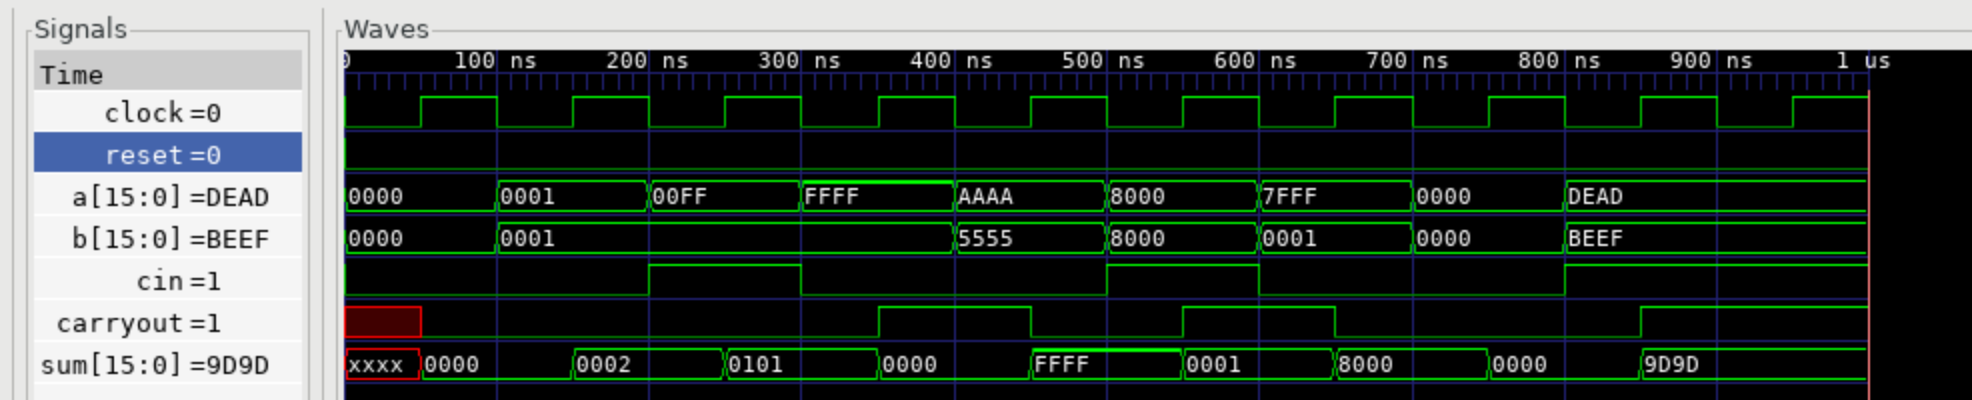
\includegraphics[width=0.95\textwidth]{pre_synthesis.png}
	\caption{GTKWave waveform before synthesis}
\end{figure}

\section{Synthesis Reports}

\subsection{Area Report}
\begin{figure}[htbp!]
	\centering
	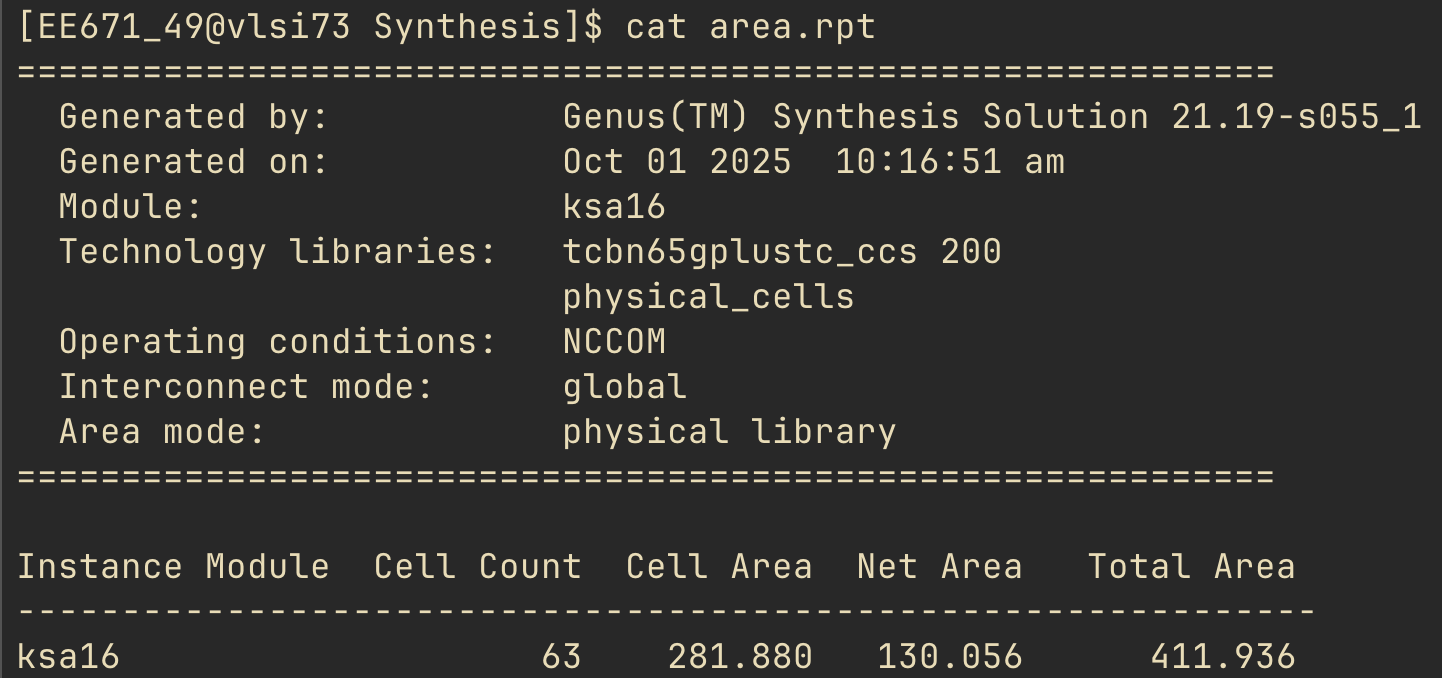
\includegraphics[width=0.95\textwidth]{area_report.png}
	\caption{Area report after synthesis}
\end{figure}

\clearpage

\subsection{Summary Report}
\begin{figure}[htbp!]
	\centering
	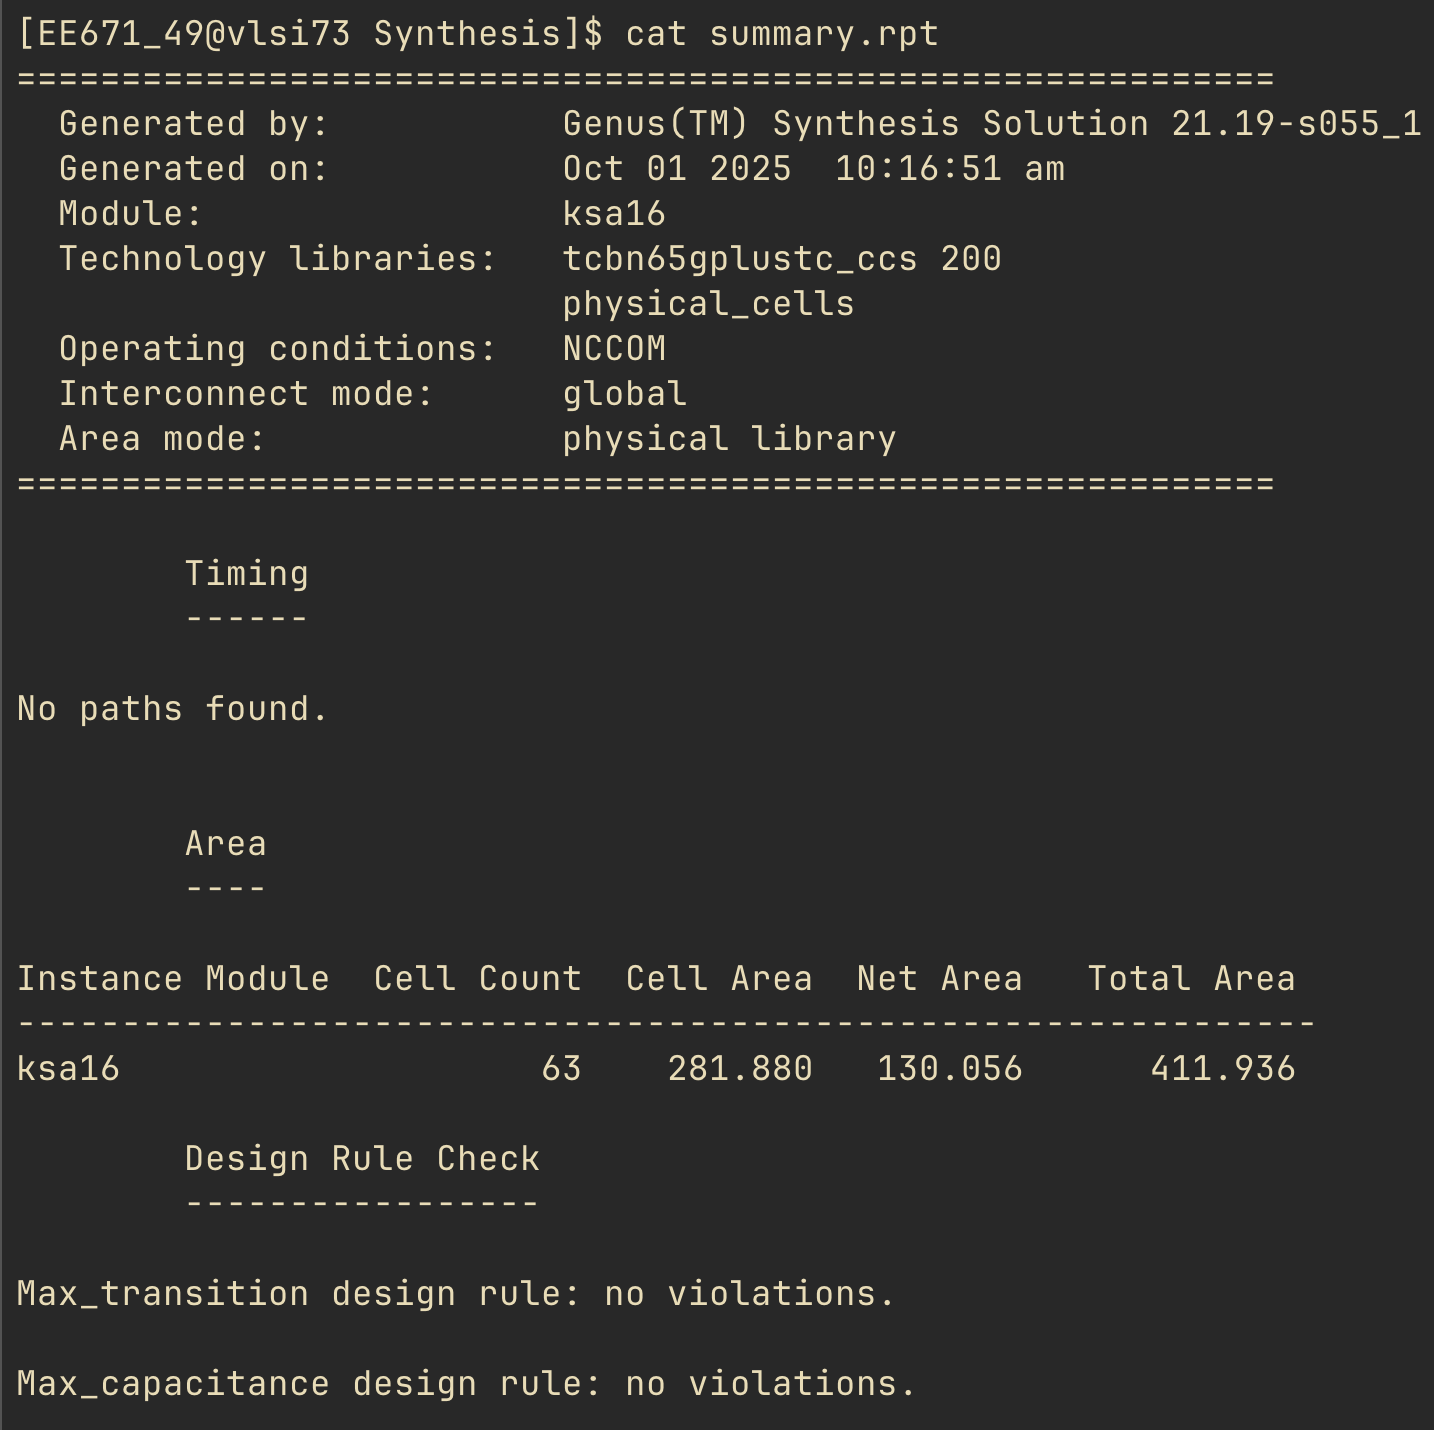
\includegraphics[width=0.95\textwidth]{summary_report.png}
	\caption{Summary report after synthesis}
\end{figure}

\subsection{Cell Count Summary}
\begin{table}[htbp!]
	\centering
	\caption{Cell statistics from RTL synthesis}
	\begin{tabular}{l c}
		\toprule
		\textbf{Parameter}                      & \textbf{Count} \\
		\midrule
		Number of Combinational Cells           & 46             \\[3pt]
		Number of Sequential Cells (Flip-Flops) & 17             \\[3pt]
		Total Number of Cells                   & 63             \\[3pt]
		\bottomrule
	\end{tabular}
\end{table}

\section{Post-Synthesis Waveform}
\begin{figure}[htbp!]
	\centering
	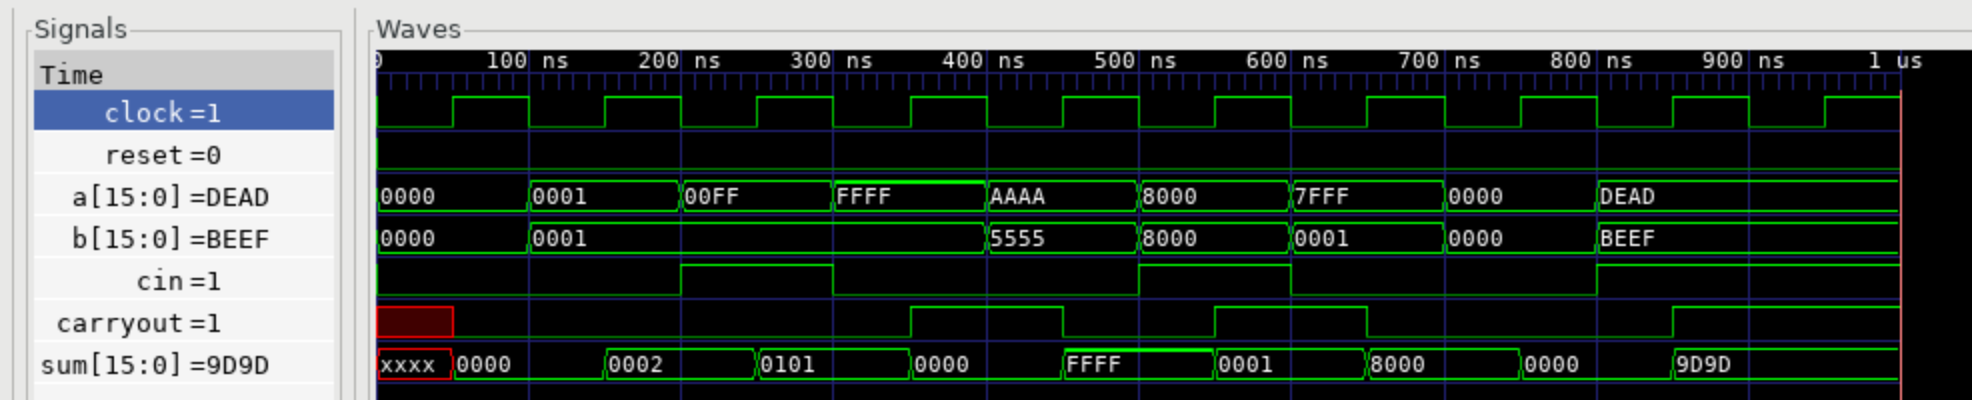
\includegraphics[width=0.95\textwidth]{post_synthesis.png}
	\caption{GTKWave waveform after synthesis}
\end{figure}

\end{document}
